\documentclass[12pt,a4paper]{article}
\usepackage{cmap}
\usepackage{amsmath}
\usepackage{amsfonts}
\usepackage{mathtext}
\usepackage{titlesec}
\usepackage{float}
\usepackage{subcaption}
\usepackage{amssymb}
\usepackage{tikz}
\usetikzlibrary{positioning, arrows.meta, shapes.geometric}
\usepackage[utf8]{inputenc}
\usepackage[T2A]{fontenc}
\usepackage{wrapfig}
\usepackage[english, russian]{babel}
\usepackage[left=2cm,right=2cm,top=2cm,bottom=2cm]{geometry}
\usepackage{indentfirst}

\DeclareSymbolFont{T2Aletters}{T2A}{cmr}{m}{it}

%%% Работа с картинками
\usepackage{graphicx}  % Для вставки рисунков
\graphicspath{{imgs/}}  % папки с картинками

\usepackage{caption}
\captionsetup{labelsep=period, labelfont=bf}

\titleformat{\section}[block]
{\normalfont}{\thesection.}{0 cm}{}
\titleformat{\subsection}[block]
{\bfseries}{\thesubsection.}{0 cm}{}

\titlespacing{\section}{17pt}{14pt}{10pt}
\titlespacing{\subsection}{17pt}{14pt}{4pt}

\def \TITLE {Отчет о выполнении лабораторной работы №9}
\def \SUBTITLE {Изучение характеристик баллистической установки}
\def \AUTHOR {Выполнил студент группы Б03-405\\ Тимохин Даниил}
\def \DATE {16 февраля 2026 г.}

\begin{document}

\begin{titlepage}
	\centering
	\vspace{5cm}
	{\scshape\large Московский физико-технический институт \\
	(НАЦИОНАЛЬНЫЙ ИССЛЕДОВАТЕЛЬСКИЙ УНИВЕРСИТЕТ)}
	
	\vspace{4cm}
	{\LARGE \TITLE}
	
	\vspace{1cm}
	{\Huge\bf \SUBTITLE }
	
	\vspace{1cm}
	\vfill
	
\begin{flushright}
	{\LARGE \AUTHOR}
\end{flushright}
	

	\vfill

	\DATE
\end{titlepage}

\newpage

\fontsize{12}{14}\selectfont

\section{ Аннотация}
Изучается зависимость скорости на выходе от начального давления и массы самого разгоняемого объекта. Также проверяется подтверждается ли теория.


\section{ Теоретическая справка}
В установке газ под давлением разгоняет тело, при этом расширяется. Из-за этого его давление падает и эффективность разгона уменьшается. Из закона сохранения энергии 

\begin{equation}
    \frac{2}{\gamma-1}a^2+u^2=\frac{2}{\gamma-1}a_0^2
\end{equation}
где a - скорость звука в среде рядом с разгоняемым объектом, u - скорость объекта.

Далее в адиабатическом приближении получаем

\begin{equation}
    p_{ст}=p_0\left( 1+ \frac{\gamma-1}{2}\frac{u^2}{a_0^2-\frac{\gamma-1}{2}u^2} \right)^{-\frac{\gamma}{\gamma-1}}
\end{equation}

Немного упростим и получим

\begin{equation}
    p_{ст}=p_0\left( 1 - \frac{\gamma-1}{2}\frac{u^2}{a_0^2} \right)^{-\frac{\gamma}{\gamma-1}}
\end{equation}

Тогда из уравнения движения ньютона

\begin{equation}
    m\frac{du}{dt}=S(p_{ст}-p_{пр})
\end{equation}

\begin{equation}
     \frac{m}{Sp_0}\frac{du}{dt}=\left( 1 - \frac{\gamma-1}{2}\frac{u^2}{a_0^2} \right)^{-\frac{\gamma}{\gamma-1}}-\frac{p_{атм}}{p_0}\left( 1 - \frac{\gamma-1}{2}\frac{u^2}{a_0^{*2}} \right)^{-\frac{\gamma}{\gamma-1}}
\end{equation}

При этом есть два упрощения: нет внешней атмосферы($p_{атм}\ll p_0$) и разложение скобки до первого порядка

Тогда получим
\begin{equation}
    u=\frac{1}{\alpha}[1-\exp{(-2g_0 \alpha^2 x)}]^\frac{1}2{}
\end{equation}
где $g_0=\frac{Sp_0}{m}$ и $\alpha^2=\gamma/(2a_0^2)$.

Данные приближения, взятые изначально с учетом того, что сам бак с воздухом намного больше объема трубки. 

Для детектирования используется лазер, чувствительный датчик света, а также осциллограф. В ходе эксперимента меняется давление и размер пули.

\newpage

\section{ Проведение эксперимента и обработка результатов}

$T_1$ - время до начала спада значения датчика, $T_2$ - время до конца спада значения датчика, $T_a$ - среднее значение.

Скорость звука $a_0=370 м/с$, $\gamma=1.4$, $l=0.5м$ - длина трубки.

Пуля: L=11.7 мм, D=6.7 мм, m=0.6 г. 

\begin{table}[H]
    \centering
    \caption{Первый эксперимент}
    \begin{tabular}{|l|l|l|l|}
    \hline
        P, дел & $T_1$, мкс & $T_2$, мкс & $T_a$, мкс \\ \hline
        16 & 71,2 & 76 & 73,6 \\ \hline
        10 & 94 & 104 & 99 \\ \hline
        20 & 66 & 73 & 69,5 \\ \hline
        25 & 58,8 & 66 & 62,4 \\ \hline
        30 & 54,4 & 62,8 & 58,6 \\ \hline
        35 & 52,4 & 62,8 & 57,6 \\ \hline
        40 & 48,8 & 58,8 & 53,8 \\ \hline
        45 & 48 & 58 & 53 \\ \hline
        50 & 47 & 54 & 50,5 \\ \hline
        55 & 41,6 & 58 & 49,8 \\ \hline
    \end{tabular}
\end{table}

\begin{figure}[H]
    \centering
    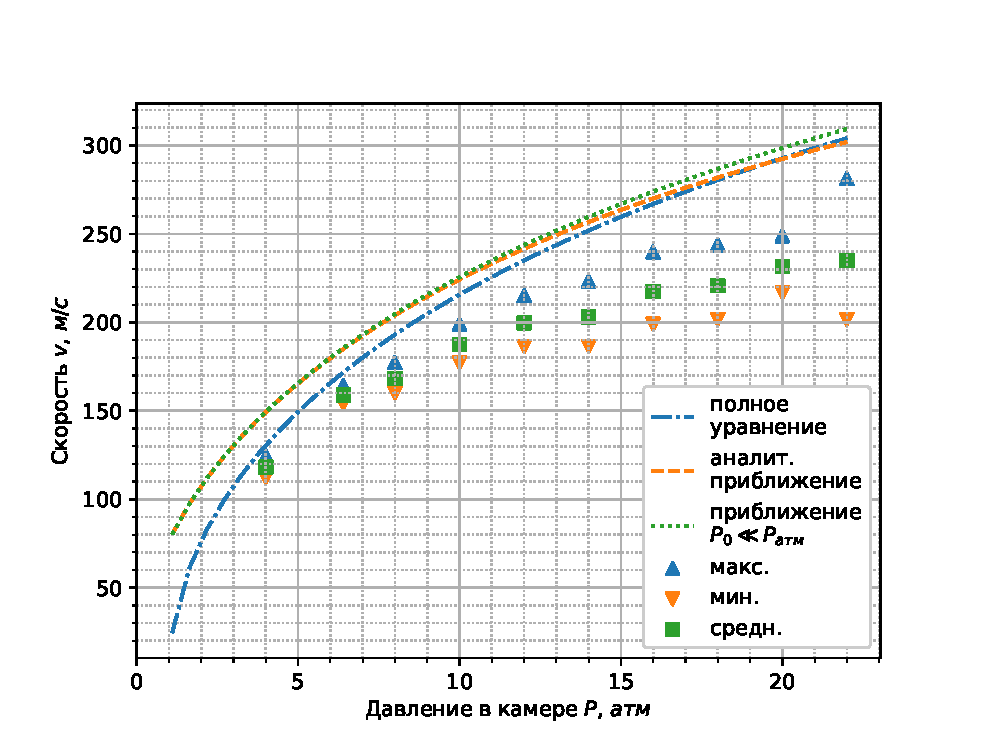
\includegraphics[width=\linewidth]{vel0.eps}
    \caption{Проверка теоретической зависимости}
\end{figure}

* "Полное уравнение" - численное интегрирование (5); "приближение $P_0\ll P_{атм}$" - численное интегрирование (5) без второго правого члена; "аналитическое приближение" - уравнение (6)


Пуля: L=7.2 мм, D=6.3 мм, m=0.3 г. 

\begin{table}[H]
    \centering
    \caption{Второй эксперимент}
    \begin{tabular}{|l|l|l|l|}
    \hline
        P, дел & $T_1$, мкс & $T_2$, мкс & $T_a$, мкс \\ \hline
        10 & 43 & 51 & 47 \\ \hline
        15 & 34 & 36,4 & 35,2 \\ \hline
        20 & 30 & 34 & 32 \\ \hline
        25 & 24,4 & 29,2 & 26,8 \\ \hline
        30 & 23,2 & 28 & 25,6 \\ \hline
        35 & 21 & 26 & 23,5 \\ \hline
        40 & 18,4 & 24 & 21,2 \\ \hline
        45 & 14 & 23 & 18,5 \\ \hline
        50 & 18,4 & 23,6 & 21 \\ \hline
    \end{tabular}
\end{table}

\begin{figure}[H]
    \centering
    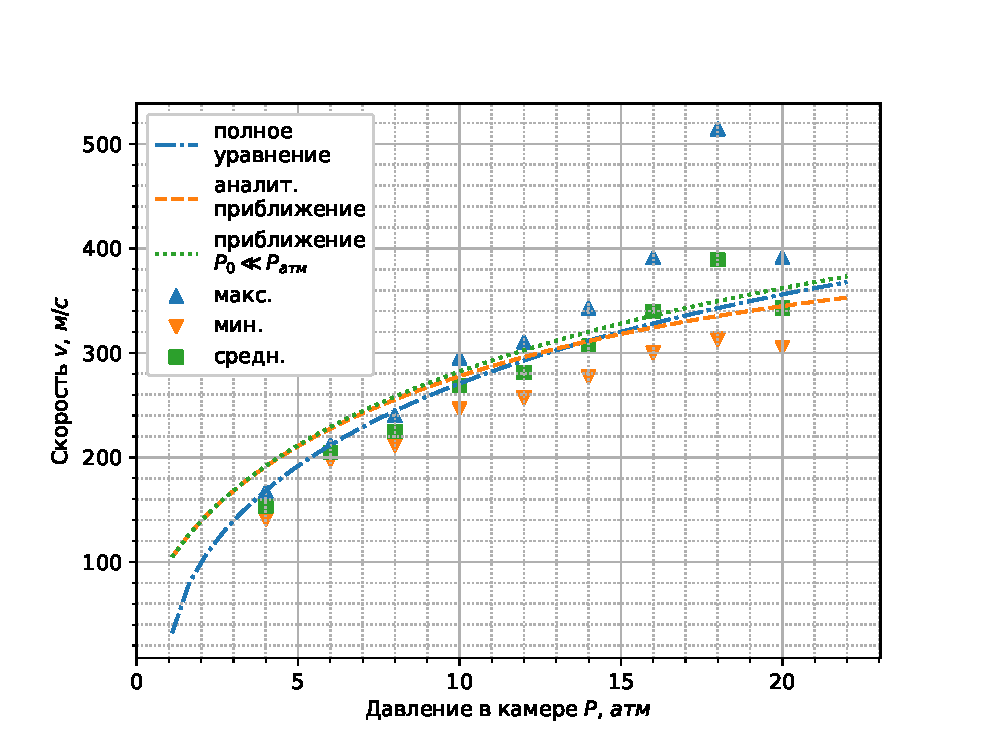
\includegraphics[width=\linewidth]{vel1.eps}
    \caption{Проверка теоретической зависимости}
\end{figure}


\section{ Обсуждение результатов и выводы}
Из результатов мы можем видеть, что теория хорошо предсказывает верхнюю границу скорости самого снаряда. Теория подтверждается лучше всего для легкой пульки.





\end{document}
